\chapter{Synthetic Graph Generation for Feature Isolation}

To better understand the underlying reasons for the small separators observed in road networks, we investigate the influence of specific graph properties in isolation.
This chapter details our approach to generating synthetic graph classes that exhibit selected features characteristic of road networks, such as low average degree, specific degree distributions, or properties related to planarity and locality.
By analyzing the separator sizes within these synthetic graphs, we aim to determine which properties, or combinations thereof, are crucial for enabling small separators.
We explore properties including, degree distribution, locality, planarity and hierarchical structure.

\section{Degree Distribution}

Our initial focus is on isolating the effect of the degree distribution.
Road networks are known to be sparse graphs.
The specific PTV Europe road network dataset \cite{ptv_group_dimacs-europe_2009} utilized in our experiments exhibits a average vertex degree of approximately \(2.47\).
A detailed visualization of the degree distribution for this network is provided in \cref{fig:degree_dist_europe}.

\begin{figure}
	\centering
	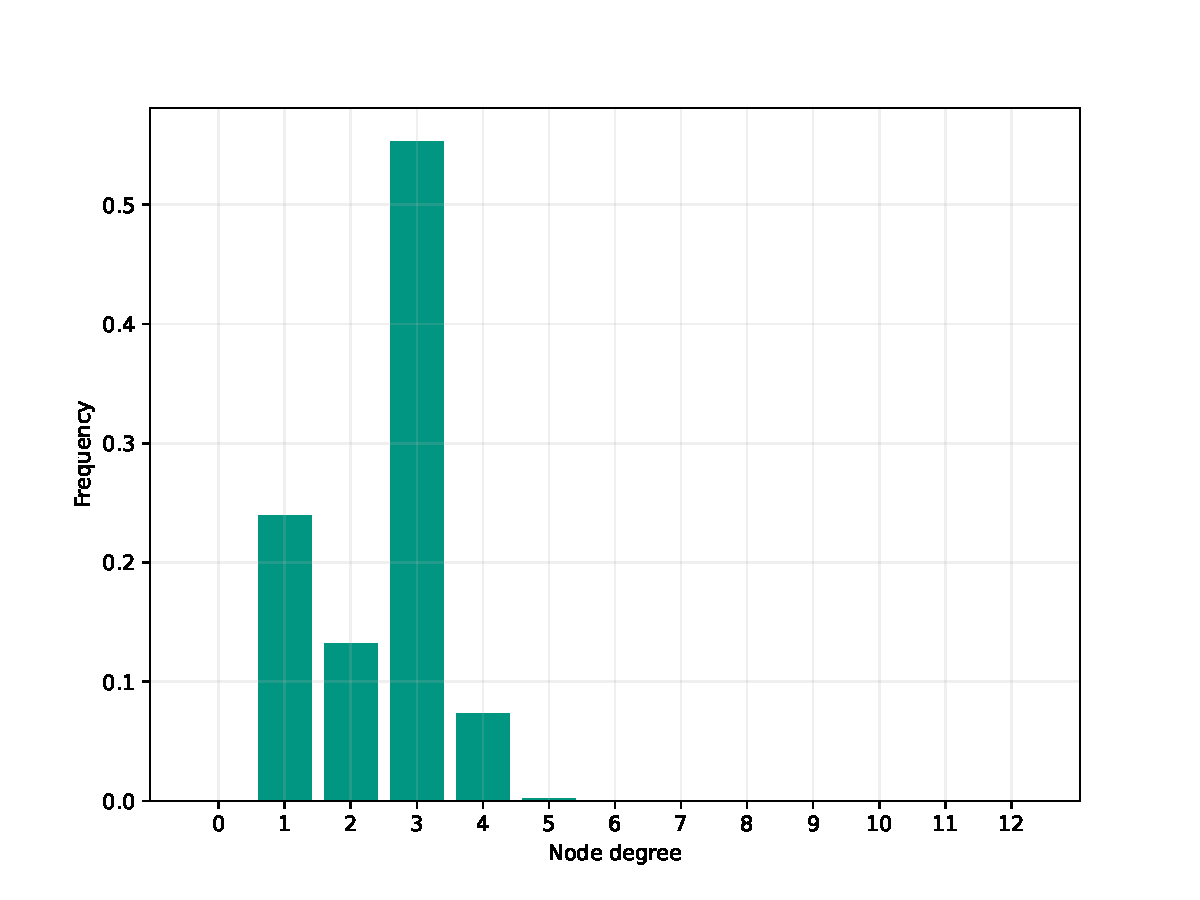
\includegraphics[width=0.6\linewidth]{graphics/degree_overview_europe.pdf}
	\caption{Degree distribution of the PTV Europe road network. The x-axis represents the vertex degree, and the y-axis shows the fraction of vertices with that degree. A single node with degree 12 has the highest degree.}
	\label{fig:degree_dist_europe}
\end{figure}

To examine whether this low average degree alone is sufficient to yield small separators, we generated connected random graphs matching this average degree.
The generation process involved two main steps.
First, a random spanning tree was created for a given set of \(n\) vertices using the algorithm described by Broder \cite{broder_generating_1989}.
This algorithm performs a random walk starting from an arbitrary vertex on the complete graph of \(n\) vertices.
An edge is marked as part of the spanning tree the first time a vertex is discovered via that edge during the walk.
The process continues until all vertices have been visited, resulting in a uniformly sampled random spanning tree in expected time \bigO{n \log n}.

It is noteworthy that random trees generated in this manner exhibit properties distinct from those of road networks.
For instance, the diameter of such random trees is known to be in \bigO{n^{1/2}} \cite{chlamtac_tree-based_1987}.
This contrasts sharply with empirical observations on road networks, such as subgraphs from the nested dissection of the Karlsruhe graph, where the diameter appears significantly smaller, estimated empirically as \bigO{n^{0.3737}}.
This observed diameter growth is visualized in \cref{fig:diameter_karlsruhe}.

\begin{figure}
	\centering
	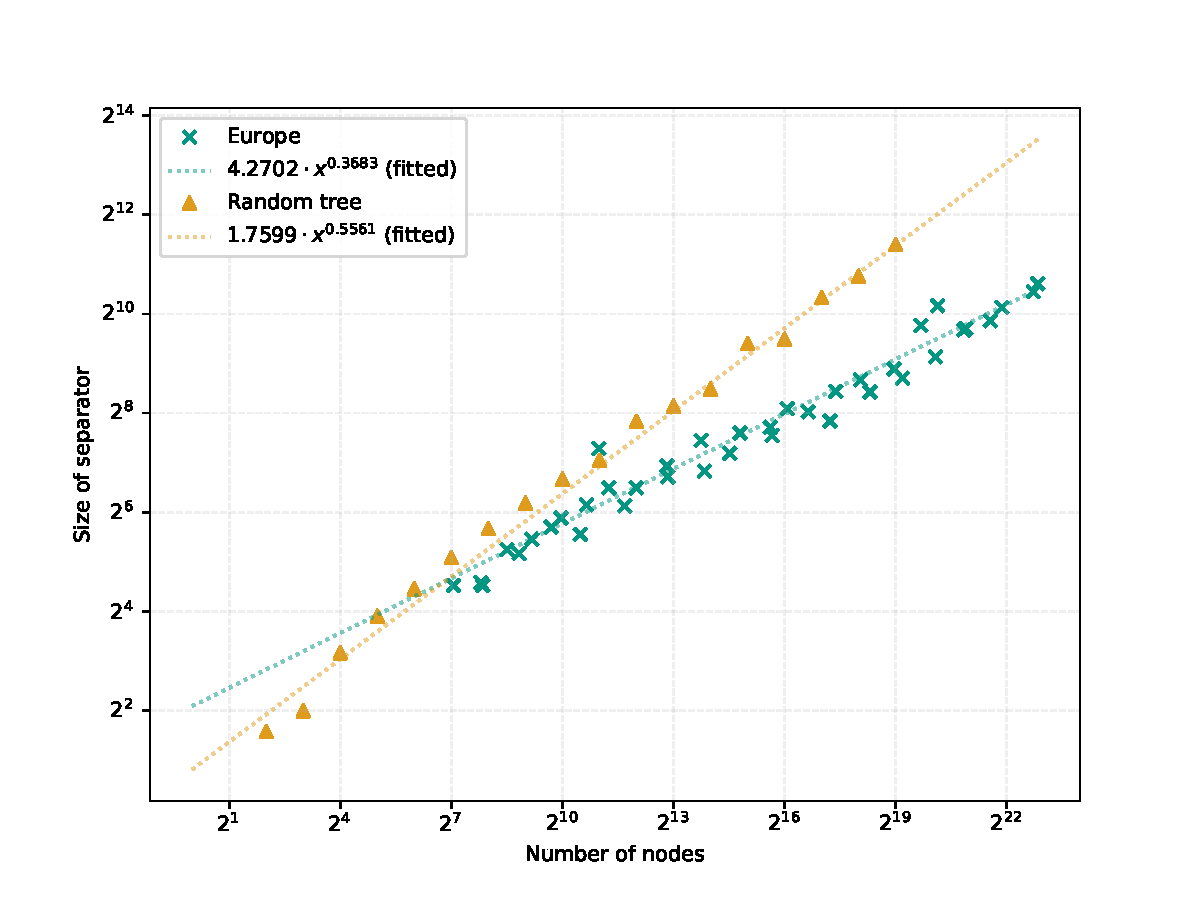
\includegraphics[width=0.6\linewidth]{graphics/diameters.pdf}
	\caption{Empirical diameter growth observed in the Karlsruhe road network subgraph. The plot shows the diameter (y-axis) as a function of the number of nodes \(n\) (x-axis, log scale).}
	\label{fig:diameter_karlsruhe}
\end{figure}

Following the generation of the initial random spanning tree, we proceeded to the second step: adding edges randomly between pairs of non-adjacent vertices.
This edge addition continued until the target average degree of \(2.47\) was reached for the entire graph.
The resulting graphs, by construction, lack the inherent locality often present in road networks.
A consequence of adding these random edges was a significant decrease in the graph diameter.
For example, graphs generated with one million nodes using this method exhibited diameters of approximately 40.

These synthetic graphs did not replicate the small separator sizes observed in real-world road networks.
Experiments yielded very large separators, with sizes scaling as \bigO{n^2}, as illustrated in \cref{fig:same_degree}.

\begin{figure}
	\centering
	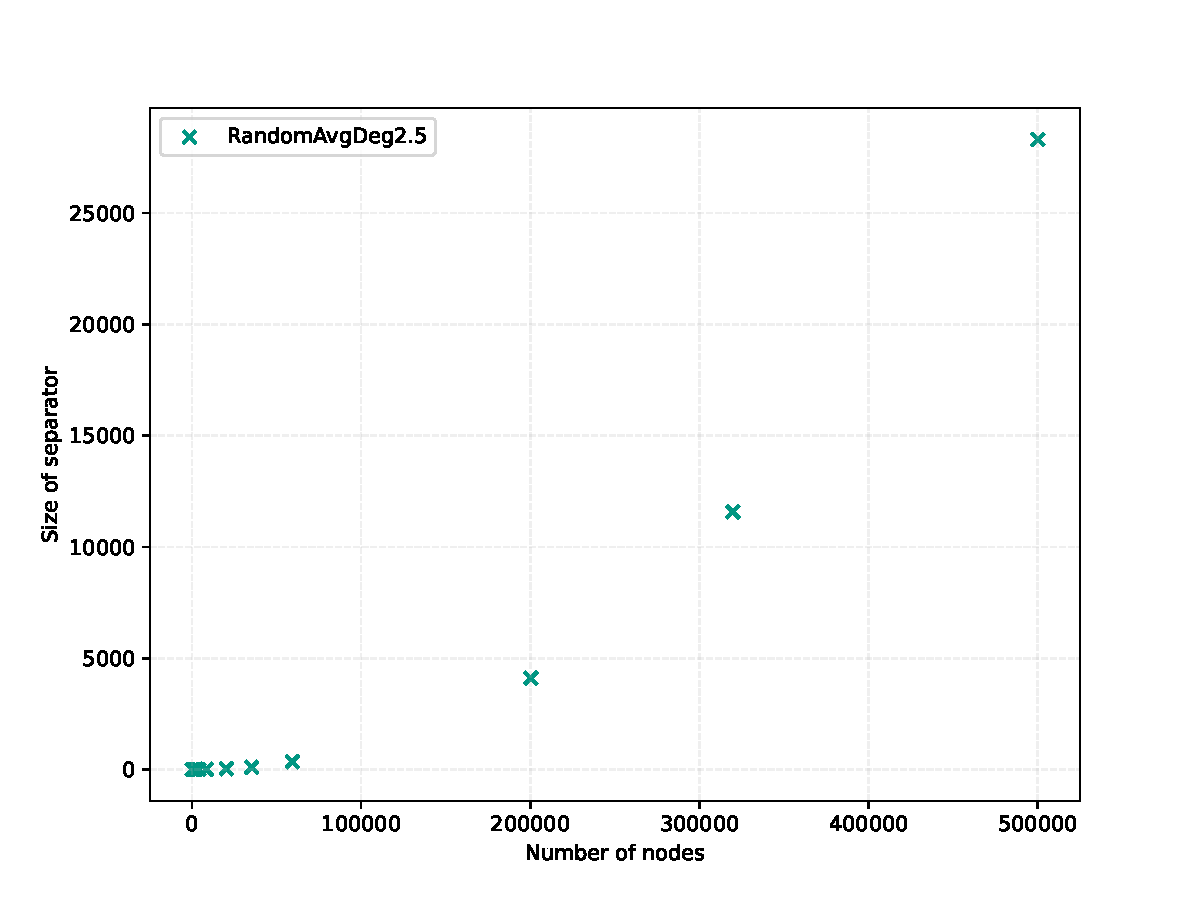
\includegraphics[width=0.6\linewidth]{graphics/RandomAvgDeg2.5.pdf}
	\caption{Separator sizes observed in random graphs generated with an average degree matching the PTV Europe road network (\( \approx 2.5 \)). The observed separator sizes are significantly larger than those found in actual road networks and scale as \bigO{n^2}.}
	\label{fig:same_degree}
\end{figure}

We also conducted experiments generating graphs that matched not just the average degree, but the specific degree distribution of the reference road network.
This involved a similar process of starting with a random tree and adding edges randomly.
However, edge addition was constrained: an edge \( (u, v) \) was only added if adding it would not cause either vertex \(u\) or \(v\) to exceed the count allocated for their respective degrees according to the target distribution sampled from the road network.
The results obtained from this refined approach were largely similar to those using only the average degree constraint.
The generated graphs continued to exhibit large separators, reinforcing the conclusion drawn from the average-degree matching experiments.

These findings suggest that the degree distribution alone is likely insufficient on its own to explain the empirically observed small separators.
Nevertheless, the low average degree remains an important factor.
Intuitively, sparser graphs, possessing fewer edges overall, should generally be easier to partition compared to denser graphs.

\section{Locality}
\label{sec:synthetic:locality}


Building upon the previous experiments focused solely on degree distribution, we maintained the core methodology of first generating a random spanning tree and then augmenting it with additional edges to achieve a desired average degree.
The crucial difference in the approach detailed in this section lies in the edge augmentation phase: we introduced constraints intended to promote locality.
This modification reflects the inherent spatial structure of road networks, where connections predominantly link geographically proximate locations.
Two distinct strategies for introducing locality during edge addition were explored.

Our first approach attempted to simulate locality based on distances within the initial random spanning tree structure.
As before, we began by generating a random spanning tree using Broder's algorithm \cite{broder_generating_1989}.
Subsequently, edges were added between non-adjacent vertices until a target average degree, chosen as \(2.5\) to approximate that of road networks, was achieved.
To incorporate locality, the probability of adding an edge between two vertices \(u\) and \(v\) was made dependent on their distance \( \text{dist}_T(u, v) \) within the initial spanning tree \(T\).
Specifically, we selected a random vertex \(x\) and chose a second vertex \(y\) with a probability related to \(f(\text{dist}_T(x, y))\), where \(f\) is a decreasing function.

Experiments using functions such as \( f(\text{dist}) = 1/\text{dist} \) resulted in graphs that still exhibited large separators.
Conversely, using rapidly decaying functions like \( f(\text{dist}) = 2^{-\text{dist}} \) led to separators of almost constant size, likely due to the graph structure remaining very close to the initial tree.
While it might be possible to fine-tune a specific function \(f\) to yield separators scaling approximately as \bigO{n^{1/3}}, such an approach risks overfitting to the target behavior without providing fundamental insights into the underlying mechanisms driving small separators in actual road networks.
Therefore, we did not pursue this direction further.

Our second approach incorporated geometric locality directly, requiring an embedding of the graph vertices in space.
We began by sampling \(n\) random points uniformly within a defined spatial domain (e.g., a unit circle).
Next, we computed the Minimum Spanning Tree (MST) of these points using Euclidean distances and Kruskal's algorithm \cite{kruskal_shortest_1956}.
Let \( \ell_{\max} \) denote the maximum edge length present in this MST.
Again to achieve the target average degree of \(2.5\), we added edges between non-adjacent vertices until the desired average degree was reached.
Crucially, these additional edges \( (u, v) \) were chosen only if their geometric distance was less than or equal to \( \ell_{\max} \).
This constraint ensures that added edges connect points that are relatively close in the geometric embedding, mimicking a form of spatial locality.
For implementation, we utilized spatial queries.
For a randomly selected vertex \(u\), we efficiently queried all other vertices \(v\) within a radius \( \ell_{\max} \) and randomly chose one to form a new edge, avoiding multi-edges and self-loops, until the target edge count was reached.

Despite incorporating this explicit geometric constraint, the resulting synthetic graphs failed to exhibit the desired separator sizes.
Our experiments indicated that separators in these geometrically generated graphs scaled with \bigO{n^{1/2}}.
This outcome is visualized in \cref{fig:geometric_locality_separators}.

\begin{figure}
	\begin{subfigure}{0.35\linewidth}
		\centering
		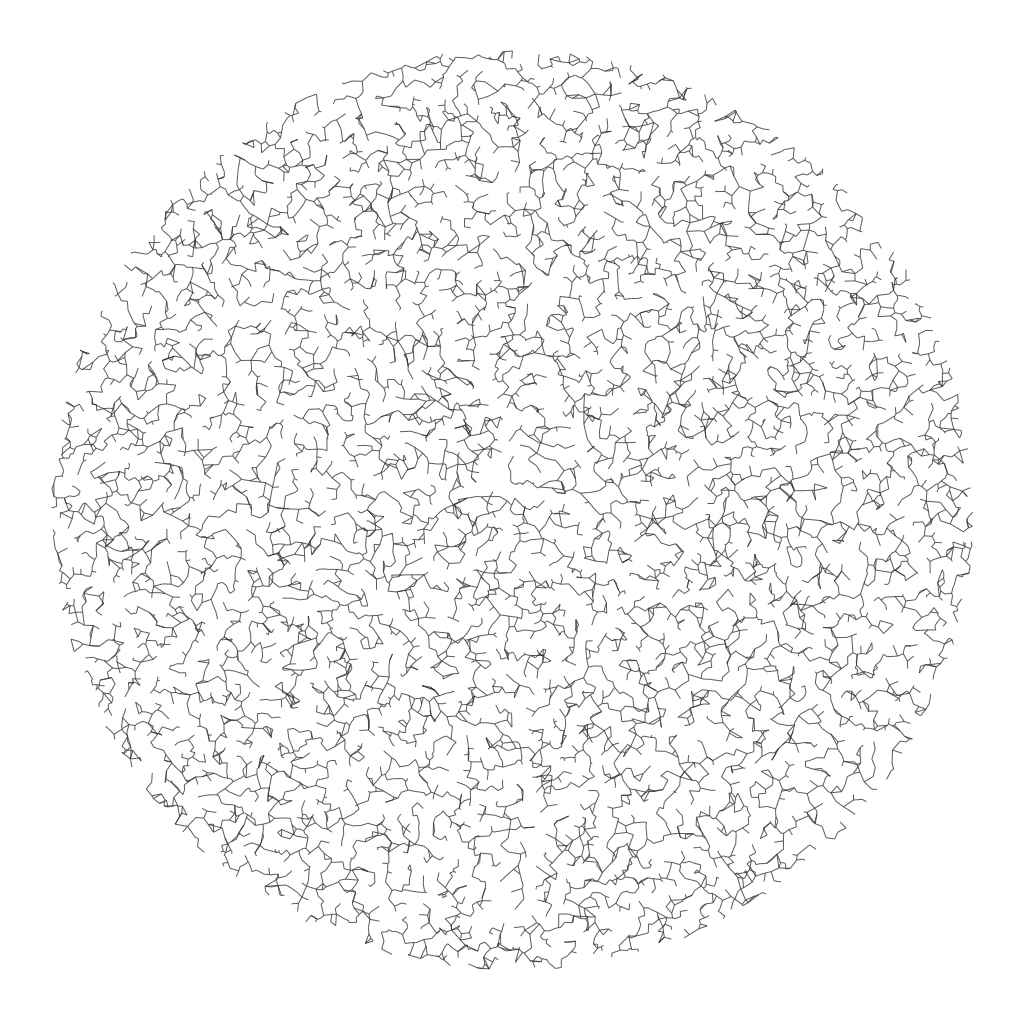
\includegraphics[width=\linewidth]{graphics/local_embedding.png}
		\caption{Visualization of a graph with 10K nodes generated using the geometric locality method.}
		\label{fig:geometric_locality_graph_viz}
	\end{subfigure}
	\hfill
	\begin{subfigure}{0.55\linewidth}
		\centering
		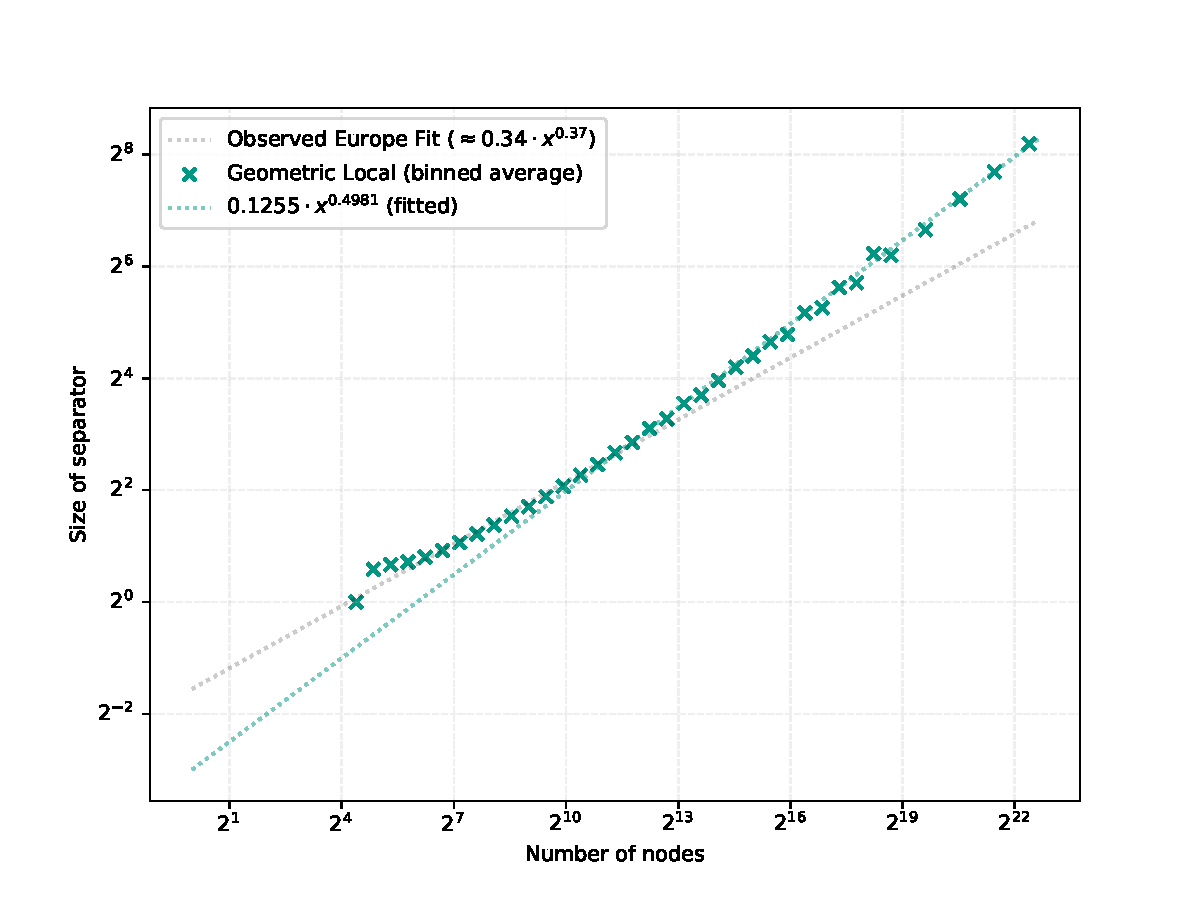
\includegraphics[width=\linewidth]{graphics/sep_local_embedding.pdf}
		\caption{Separator size scaling for synthetic graphs generated with geometric locality.}
		\label{fig:geometric_locality_sep_plot}
	\end{subfigure}
	\caption{Synthetic graph generation using geometric locality and analysis of separator sizes.}
	\label{fig:geometric_locality_separators}
\end{figure}

The results from the geometric locality approach suggest that merely combining low average degree with this specific form of locality is insufficient to reproduce the cubic root separator sizes of road networks.

\paragraph{Real-World Implications}

It is worth considering the practical implications of different asymptotic growth rates for separator sizes within the typical scale of road networks.
While \bigO{c_1\cdot n^{1/3}} and \bigO{c_2 \cdot n^{1/2}}, with \(c_2 \ll c1\) diverge significantly for large \(n\), the actual separator sizes for graphs up to around 20 million vertices are numerically similar.
The performance of algorithms leveraging graph separators in real-world applications may be more significantly influenced by the absolute sizes of separators achievable in practice, compared to the a specific scaling model.
Performance gains, for e.g. CCH could potentially be realized even if the separators behave like \(c \cdot n^{1/2}\) for a sufficiently small \(c\), as the absolute separator sizes remain manageable for networks of practical relevance.

\paragraph{Initial Deviations in Separator Scaling}

An interesting characteristic is observable for graphs with small node counts in empirical studies of road networks.
As a careful reader may have already spotted in \cref{fig:separator_size_loglog_non_binned}, real road networks often exhibit a deviation in separator scaling for graphs containing approximately \(2^6\) nodes.
\cref{fig:outlier_histograms} presents histogram plots to better visualize the prevalence of these instances for both real-world data and our synthetic model.
Specifically, \cref{fig:real_europe_hist} shows this phenomenon for European road network samples.
These plots reveal an initial peak in relative separator size for small graphs, followed by a slight decrease, before the data aligns with the more dominant scaling trend observed for larger graphs.

\begin{figure}
	\centering
	\begin{subfigure}{0.48\linewidth}
		\centering
		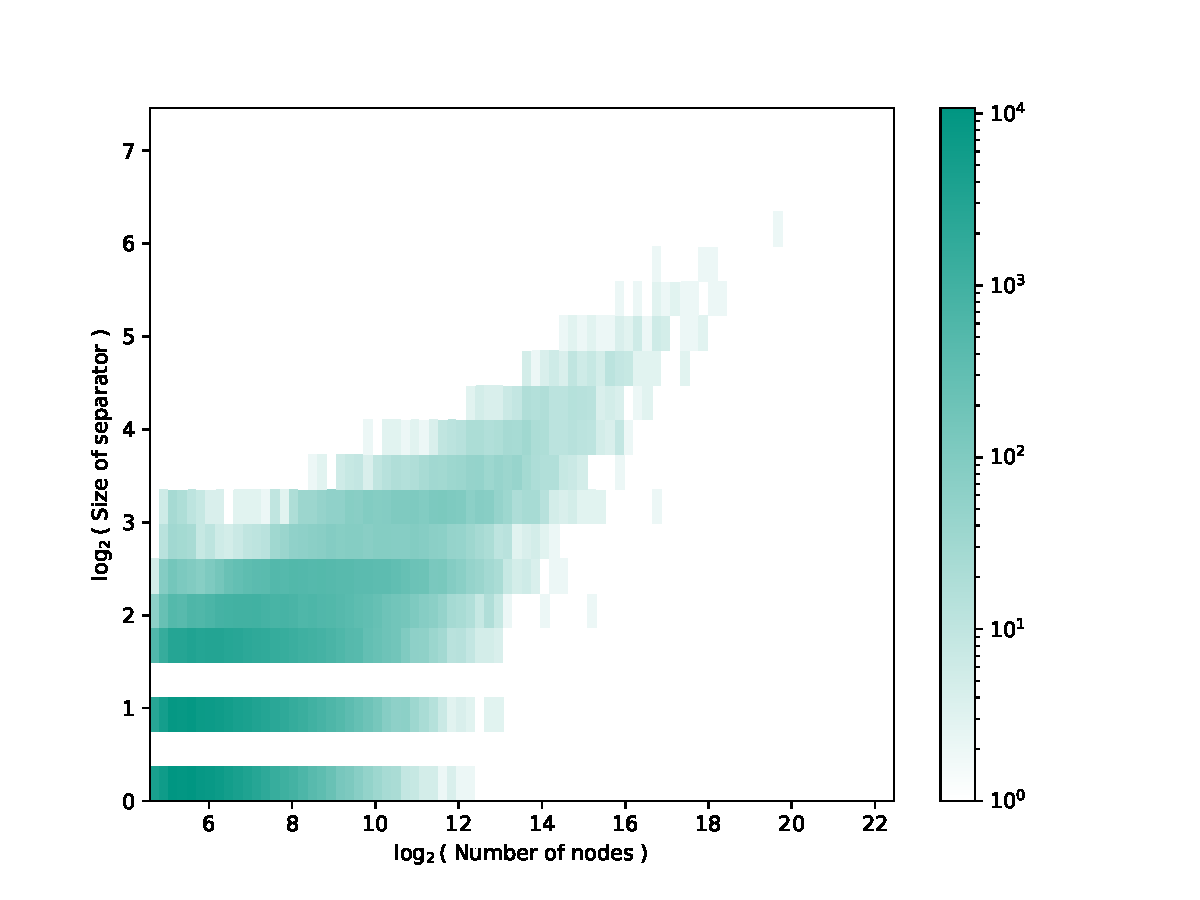
\includegraphics[width=\linewidth]{graphics/Germany-hist.pdf}
		\caption{Histogram of separator sizes for the European road network.}
		\label{fig:real_europe_hist}
	\end{subfigure}
	\hfill
	\begin{subfigure}{0.48\linewidth}
		\centering
		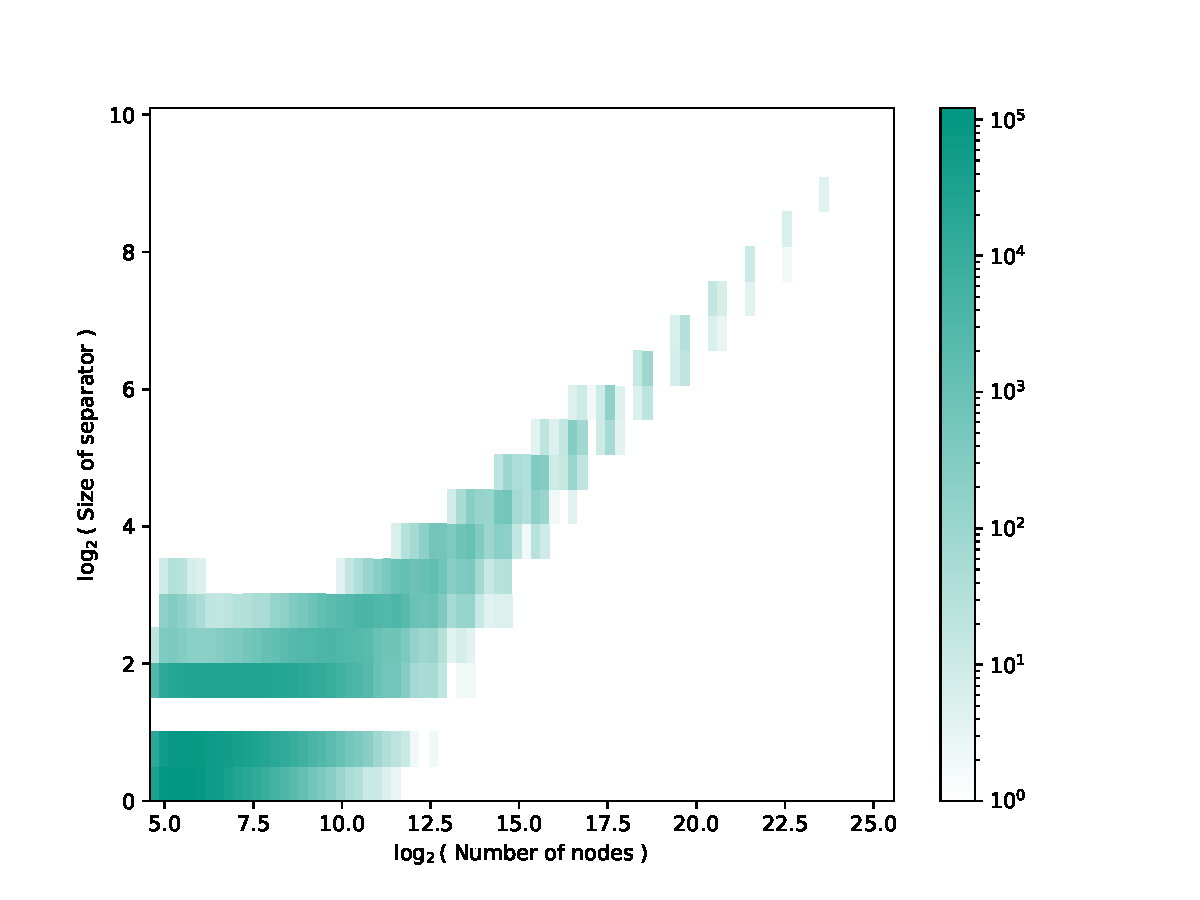
\includegraphics[width=\linewidth]{graphics/local_embedding-hist.pdf}
		\caption{Histogram of separator sizes for synthetic graphs using geometric locality.}
		\label{fig:local_embedding_hist}
	\end{subfigure}
    \caption{Histograms illustrating the distribution of separator sizes, comparing real road networks (left) and the geometric locality model (right). A slight increase in separator size is observed for graphs with \(\approx 2^6\) nodes.}
	\label{fig:outlier_histograms}
\end{figure}

Our synthetic graphs generated using the geometric locality approach exhibited a similar initial pattern, as can be discerned from the histogram in \cref{fig:local_embedding_hist}.
This initial behavior in the synthetic model appears qualitatively comparable, although slightly more pronounced than in the real network data.
This correspondence is noteworthy.
It suggests that the geometric locality model, despite failing to replicate the overall asymptotic separator scaling of \bigO{n^{1/3}}, may capture certain structural properties relevant at smaller graph scales that are present in actual road networks.






\section{Planarity}
\label{sec:synthetic:planarity}

Road networks exhibit characteristics of near-planarity.
As discussed previously in \cref{sec:approach:planarity}, it is possible to model road networks as planar graphs, or achieve planarity through minor modifications, without substantially increasing separator sizes.
This approximate planarity motivates an investigation into whether standard planar graph models can replicate the separator behavior observed in road networks, particularly when constrained to have similar sparsity.
We therefore examined separator properties in two common classes of planar graphs: grids and Delaunay triangulations, modified to match the low average degree found in road networks.

Our initial investigation focused on grid graphs, a fundamental class known to possess separators scaling as \bigO{n^{1/2}}.
To align their sparsity with road networks, we generated modified grids with an average degree of approximately \(2.5\).
The generation process started with a standard two-dimensional grid graph.
Edges were then removed uniformly at random until the target average degree was reached over the entire graph.
Subsequently, we identified and utilized the largest connected component for analysis.
We observed that even without explicit mechanisms to prevent disconnection during edge removal, the largest connected component typically encompassed a very large fraction of the initial vertices.

Analysis of these sparse grid graphs revealed separator sizes consistent with the \bigO{n^{1/2}} asymptotic behavior of complete grids.
However, the constant factor associated with this scaling appeared to be relatively small.
Consequently, although the asymptotic limit behavior differs from the \bigO{n^{1/3}} scaling empirically observed for road networks, the absolute separator sizes in these sparse grids were numerically quite similar to those of road networks for graphs up to typical sizes (e.g., around 20 million nodes).
This finding highlights that sparsity, even within a simple planar structure like a grid, can lead to separators that are small in absolute terms for practical graph dimensions.
\Cref{fig:sparse_grid_separators} illustrates a sample sparse grid and the observed separator scaling.

\begin{figure}
	\centering
	\begin{subfigure}{0.35\linewidth}
		\centering
		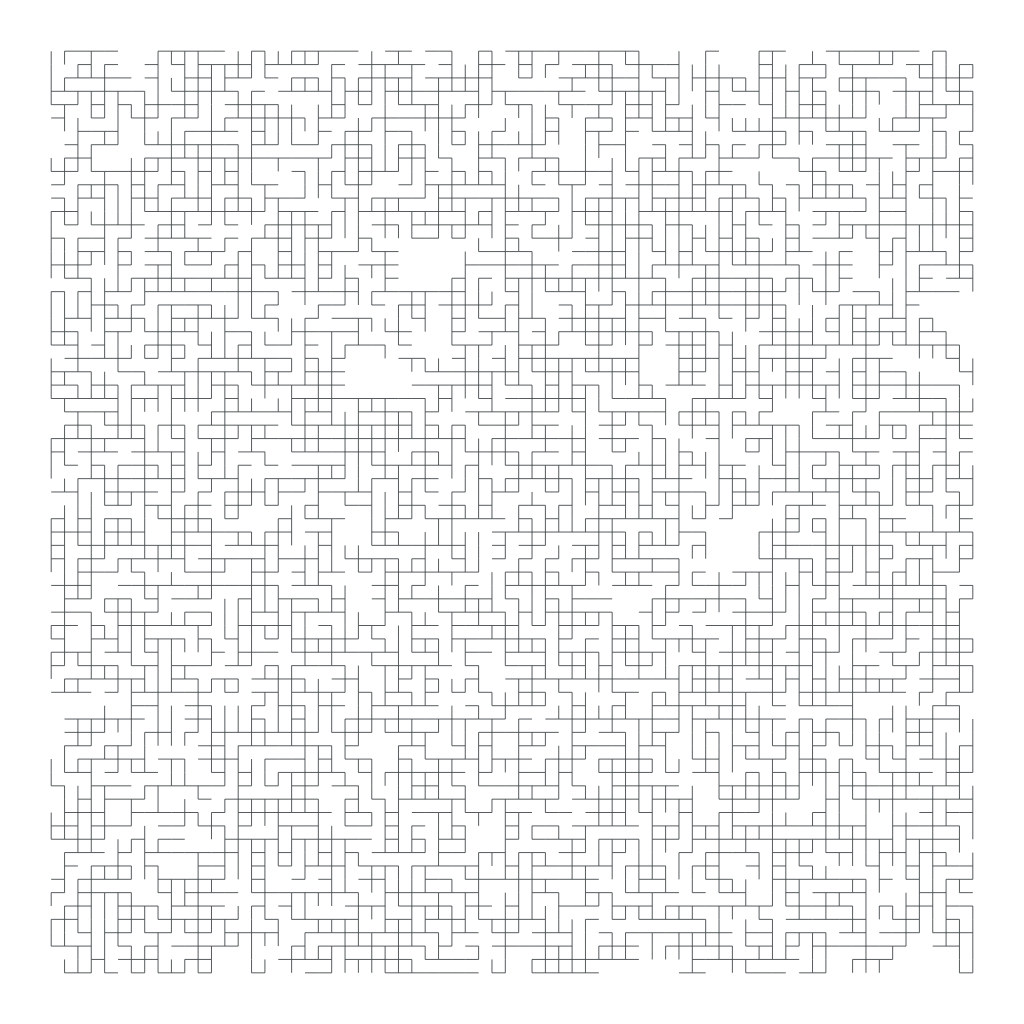
\includegraphics[width=\linewidth]{graphics/grid_avg_deg.png}
		\caption{Visualization of the largest connected component of a grid graph with \(\approx 10\text{K}\) nodes after random edge removal to achieve an average degree of \(2.5\).}
		\label{fig:sparse_grid_viz} % Specific sub-label
	\end{subfigure}
	\hfill
	\begin{subfigure}{0.55\linewidth}
		\centering
		\includegraphics[width=\linewidth]{graphics/sep_grid_avg_deg.png}
		\caption{Separator size scaling for sparse grid graphs (average degree \(2.5\)).}
		\label{fig:sparse_grid_sep_plot} % Specific sub-label
	\end{subfigure}
	\caption{Analysis of sparse grid graphs with average degree \(2.5\). (a) Example structure. (b) Separator sizes scale approximately as \bigO{n^{1/2}}, but with a small constant factor leading to absolute sizes comparable to road networks at practical scales.}
	\label{fig:sparse_grid_separators} % Main label
\end{figure}

We extended this investigation to Delaunay triangulations, which can be viewed as a generalization of grids derived from point sets.
Our process involved sampling points uniformly at random in a two-dimensional space and computing their Delaunay triangulation.
Similar to the grid experiments, we then randomly deleted edges from the triangulation until the average degree reached the target value of \(2.5\), again typically analyzing the largest connected component.

As might be expected, the results obtained from these sparse Delaunay graphs were largely analogous to those from sparse grids.
The separators exhibited scaling consistent with \bigO{n^{1/2}}, characteristic of planar graphs, yet the associated constant factors were small.
This again led to absolute separator sizes that were numerically comparable to those measured in road networks for graphs of relevant sizes.
These findings are depicted in \cref{fig:sparse_delaunay_separators}.

\begin{figure}
	\centering
	\begin{subfigure}{0.35\linewidth}
		\centering
		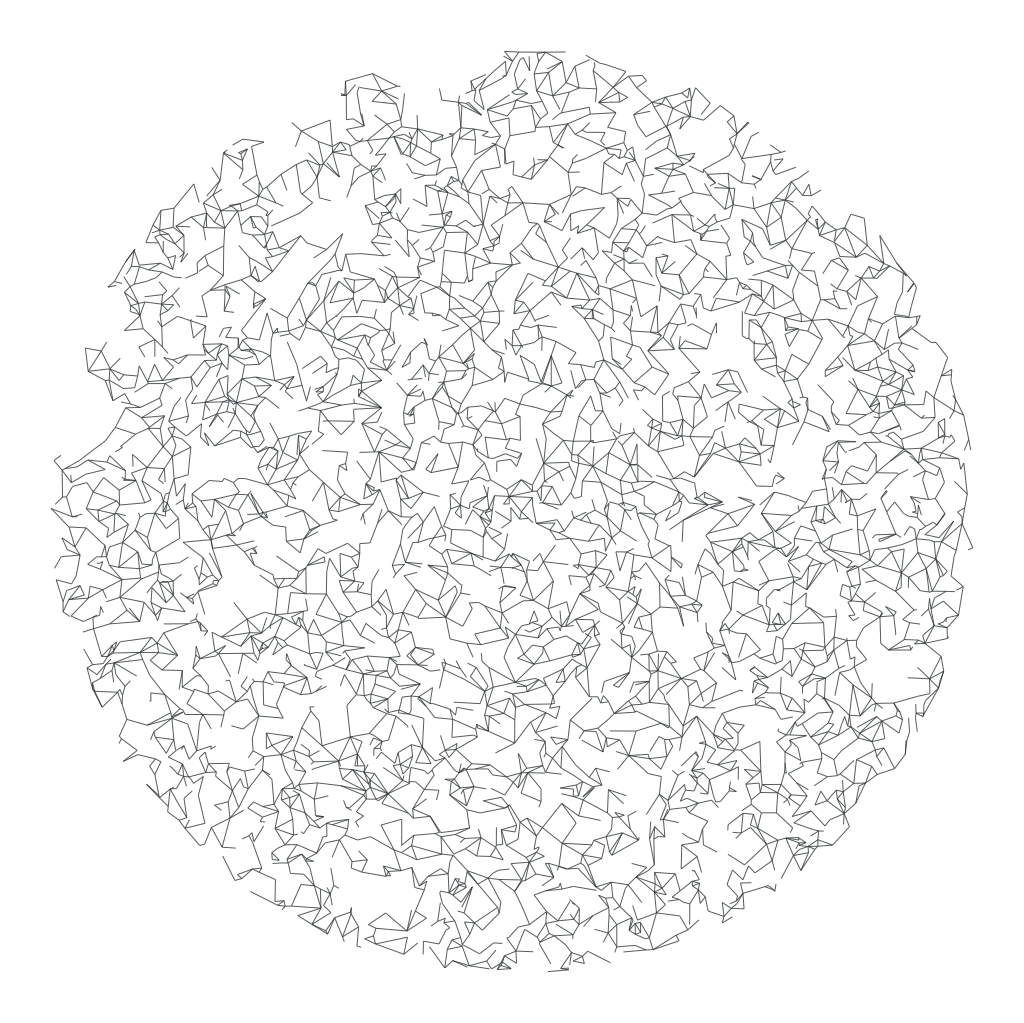
\includegraphics[width=\linewidth]{graphics/delaunay_avg_deg.png}
		\caption{Visualization of a sparse Delaunay triangulation with 5K nodes after random edge removal to achieve an average degree of \(2.5\).}
		\label{fig:sparse_delaunay_viz}
	\end{subfigure}
	\hfill
	\begin{subfigure}{0.55\linewidth}
		\centering
		\includegraphics[width=\linewidth]{graphics/sep_delaunay_avg_deg.png}
		\caption{Separator size scaling for sparse Delaunay graphs (average degree \(2.5\)). The plot shows separator size (y-axis) versus graph size \(n\) (x-axis).}
		\label{fig:sparse_delaunay_sep_plot} % Specific sub-label
	\end{subfigure}
	\caption{Analysis of sparse Delaunay graphs with average degree \(2.5\). (a) Example structure derived from random points. (b) Separator sizes scale approximately as \bigO{n^{1/2}} with small constant factors, yielding absolute sizes similar to road networks at practical scales.}
	\label{fig:sparse_delaunay_separators} % Main label
\end{figure}

The experiments with sparse grids and Delaunay triangulations suggest that combining planarity with low average degree results in graphs whose practical separator sizes are surprisingly close to those of road networks, despite potentially differing asymptotic scaling.

\section{Highway Dimension}
\label{sec:synthetic:highway_dimension}

Given that the simpler graph models explored in previous sections did not reproduce the observed \bigO{n^{1/3}} separator scaling of road networks, we turned our attention to more complex generative processes designed to capture other relevant structural properties.
One such property is highway dimension, introduced by Abraham et al. \cite{abraham_highway_2010}.
Intuitively, a graph possesses a small highway dimension if, for every radius \(r > 0\), there exists a sparse set of vertices \(S_r\) such that every shortest path longer than \(r\) intersects \(S_r\).
A set is considered sparse if every ball of radius \(\mathcal{O}(r)\) contains only a small number of vertices from \(S_r\) \cite{abraham_highway_2010}.
The significance of this property stems from the finding that low highway dimension provides provable performance guarantees for several important route planning algorithms, including REACH \cite{goldberg_reach_2006}, Contraction Hierarchies \cite{geisberger_contraction_2008}, Highway Hierarchies \cite{sanders_highway_2005}, Transit Node Routing \cite{bast_fast_2007}, and SHARC \cite{bauer_sharc_2010}.

The work introducing highway dimension also proposed a synthetic graph generator (henceforth ABR generator) intended to produce graphs exhibiting this property \cite{abraham_highway_2010}.
A good explanation of the generation process is provided in \cite{hutchison_synthetic_2010}, which we summarize here.
The generation process operates iteratively.
It begins with an empty graph \( G = (V, E) = (\emptyset, \emptyset) \) and progressively adds new vertices \(v_t\) to \(V\), whose locations in the metric space are chosen randomly.
Throughout this process, the generator maintains a series of \(2^i\)-covers, denoted \(C_i\), for each level \(i\) where \(1 \leq i \leq \log D\), and \(D\) represents the diameter of the metric space.
A set \(C_i \subseteq V\) is a \(2^i\)-cover if any two vertices \(u, v \in C_i\) satisfy \(d(u, v) \geq 2^i\), and every vertex \(u \in V\) is within distance \(2^i\) of some vertex in \(C_i\).
When a new vertex \(v_t\) is added, the generator identifies the smallest index \(i\) such that there exists a vertex \(w \in C_i\) with \(d(v_t, w) \leq 2^i\).
The new vertex \(v_t\) is then added to all covers \(C_j\) for which \(0 \leq j < i\).
If no such index \(i\) exists, \(v_t\) is added to all cover sets \(C_j\).
Edges are subsequently added based on these covers and a tuning parameter \(k\).
For each cover \(C_j\) containing \(v_t\) (where \(0 \leq j < i\)), and for each existing vertex \(w \in C_j\), an edge \((w, v_t)\) is added if their distance satisfies \(d(w, v_t) \leq k \cdot 2^j\).
Furthermore, for each \(C_j\) containing \(v_t\) where \(j < \log D\) and \(v_t\) is also present in \(C_{j+1}\), an edge is added connecting \(v_t\) to its nearest neighbor within the set \(C_{j+1}\). % Note: Phrased carefully based on user input, which might contain ambiguity regarding cover membership conditions.
For our experiments, we adopted parameter settings similar to those used by \cite{hutchison_synthetic_2010}, setting the diameter \(D = 2^{25}\) and the connection parameter \(k = \sqrt{2}\).

Bauer et al. also described an alternative node sampling strategy aimed at creating structures resembling city clusters \cite{hutchison_synthetic_2010}.
We implemented and tested both the uniform random sampling and this cluster-based sampling approach.
Our experiments indicated no significant difference in the resulting separator sizes between the two sampling methods using the ABR generator framework.

The analysis of graphs generated using the ABR method yielded separators that scaled approximately as \bigO{n^{1/2}}.
This result is noteworthy because graphs generated by this process are typically highly non-planar.
It serves as a reminder that observing \bigO{n^{1/2}} separator scaling does not necessarily imply planarity.
\Cref{fig:abr_graph_separators} provides a visual example of an ABR-generated graph and illustrates the observed separator scaling.

\begin{figure}
	\centering
	\begin{subfigure}{0.35\linewidth}
		\centering
		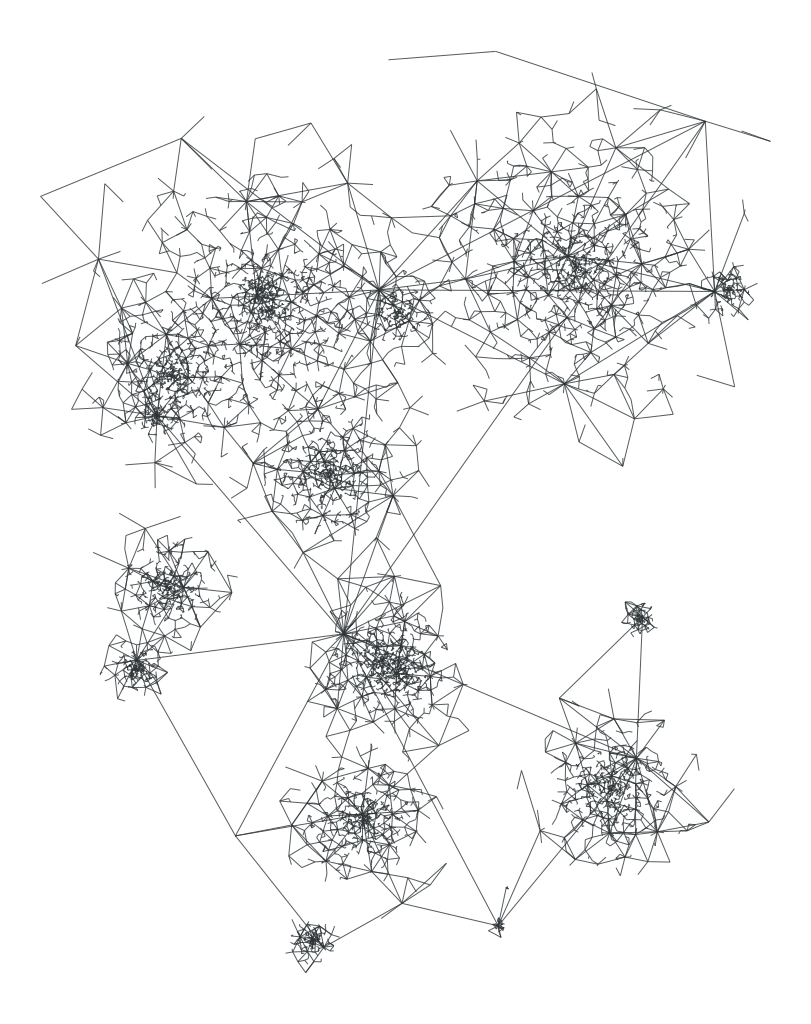
\includegraphics[height=\linewidth, angle=90]{graphics/highway.png}
		\caption{Visualization of a synthetic graph generated using the ABR low highway dimension algorithm with 10K nodes.}
		\label{fig:abr_graph_viz} % Specific sub-label
	\end{subfigure}
	\hfill
	\begin{subfigure}{0.55\linewidth}
		\centering
		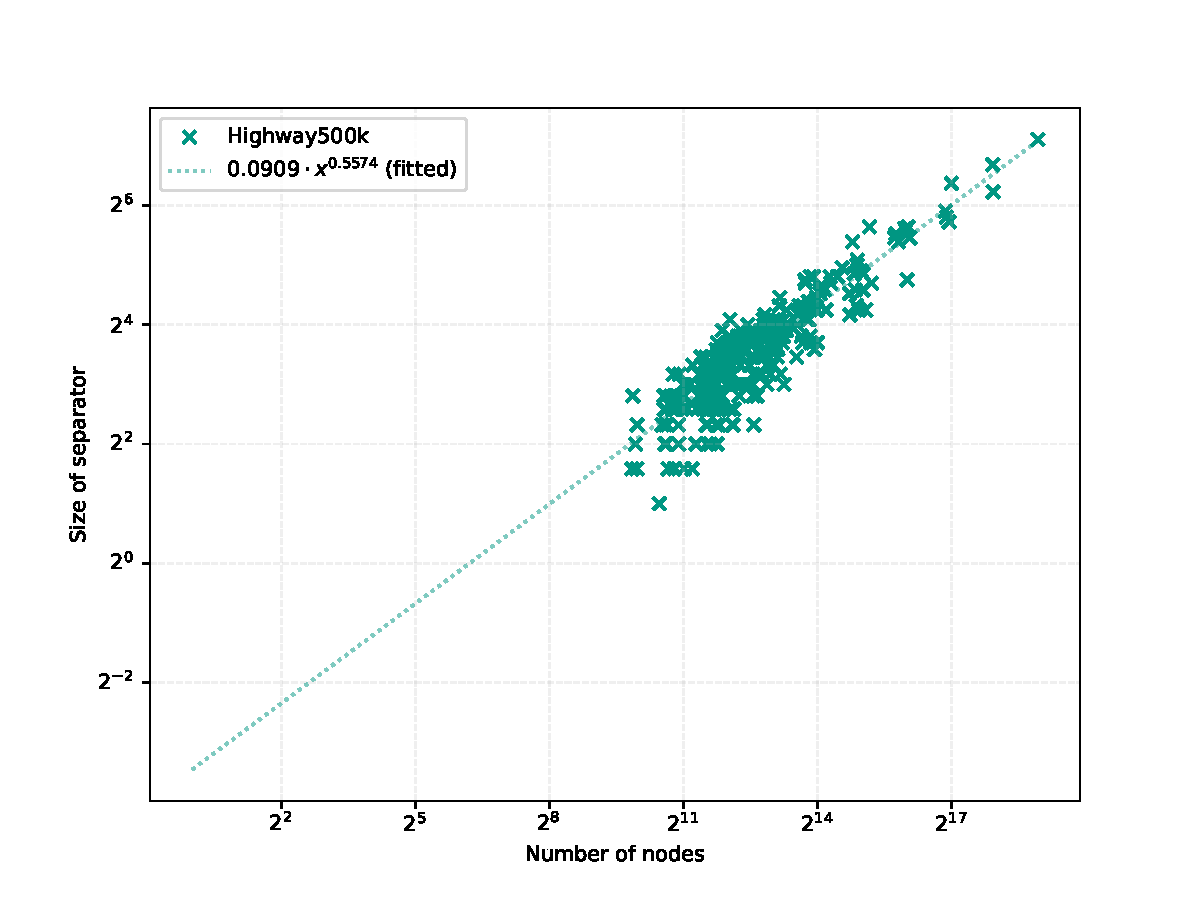
\includegraphics[width=\linewidth]{graphics/sep_highway.pdf}
		\caption{Separator size scaling observed during recursive partitioning of ABR-generated graphs.}
		\label{fig:abr_graph_sep_plot} % Specific sub-label
	\end{subfigure}
	\caption{Analysis of synthetic graphs generated using the ABR algorithm \cite{abraham_highway_2010}. (a) Example structure. (b) Separator sizes scale approximately as \bigO{n^{1/2}}.}
	\label{fig:abr_graph_separators} % Main label
\end{figure}

\section{Hierarchical Structure}
\label{sec:synthetic:hierarchical_structure}

\subsection{Nested Voronoi Diagrams / Nested Grids}
\label{sec:synthetic:nested_voronoi}

\subsection{Hierarchical Clustering}
\label{sec:synthetic:hierarchical_clustering}

